\documentclass[11pt]{article}

\usepackage{verbatim}
\usepackage{amsmath}
\usepackage{amssymb}
\usepackage{setspace}
\usepackage[top=1in, bottom=1in, left=1.25in, right=1.25in]{geometry}
\usepackage{subfigure}
\usepackage{graphicx}
\usepackage{cite}
\usepackage[squaren]{SIunits}
\usepackage{listings}
\usepackage{csquotes}

\setlength{\parindent}{0pt} 	% remove the silly paragraph indents

% Sample figure
%\begin{figure}[h!]
%\centering
%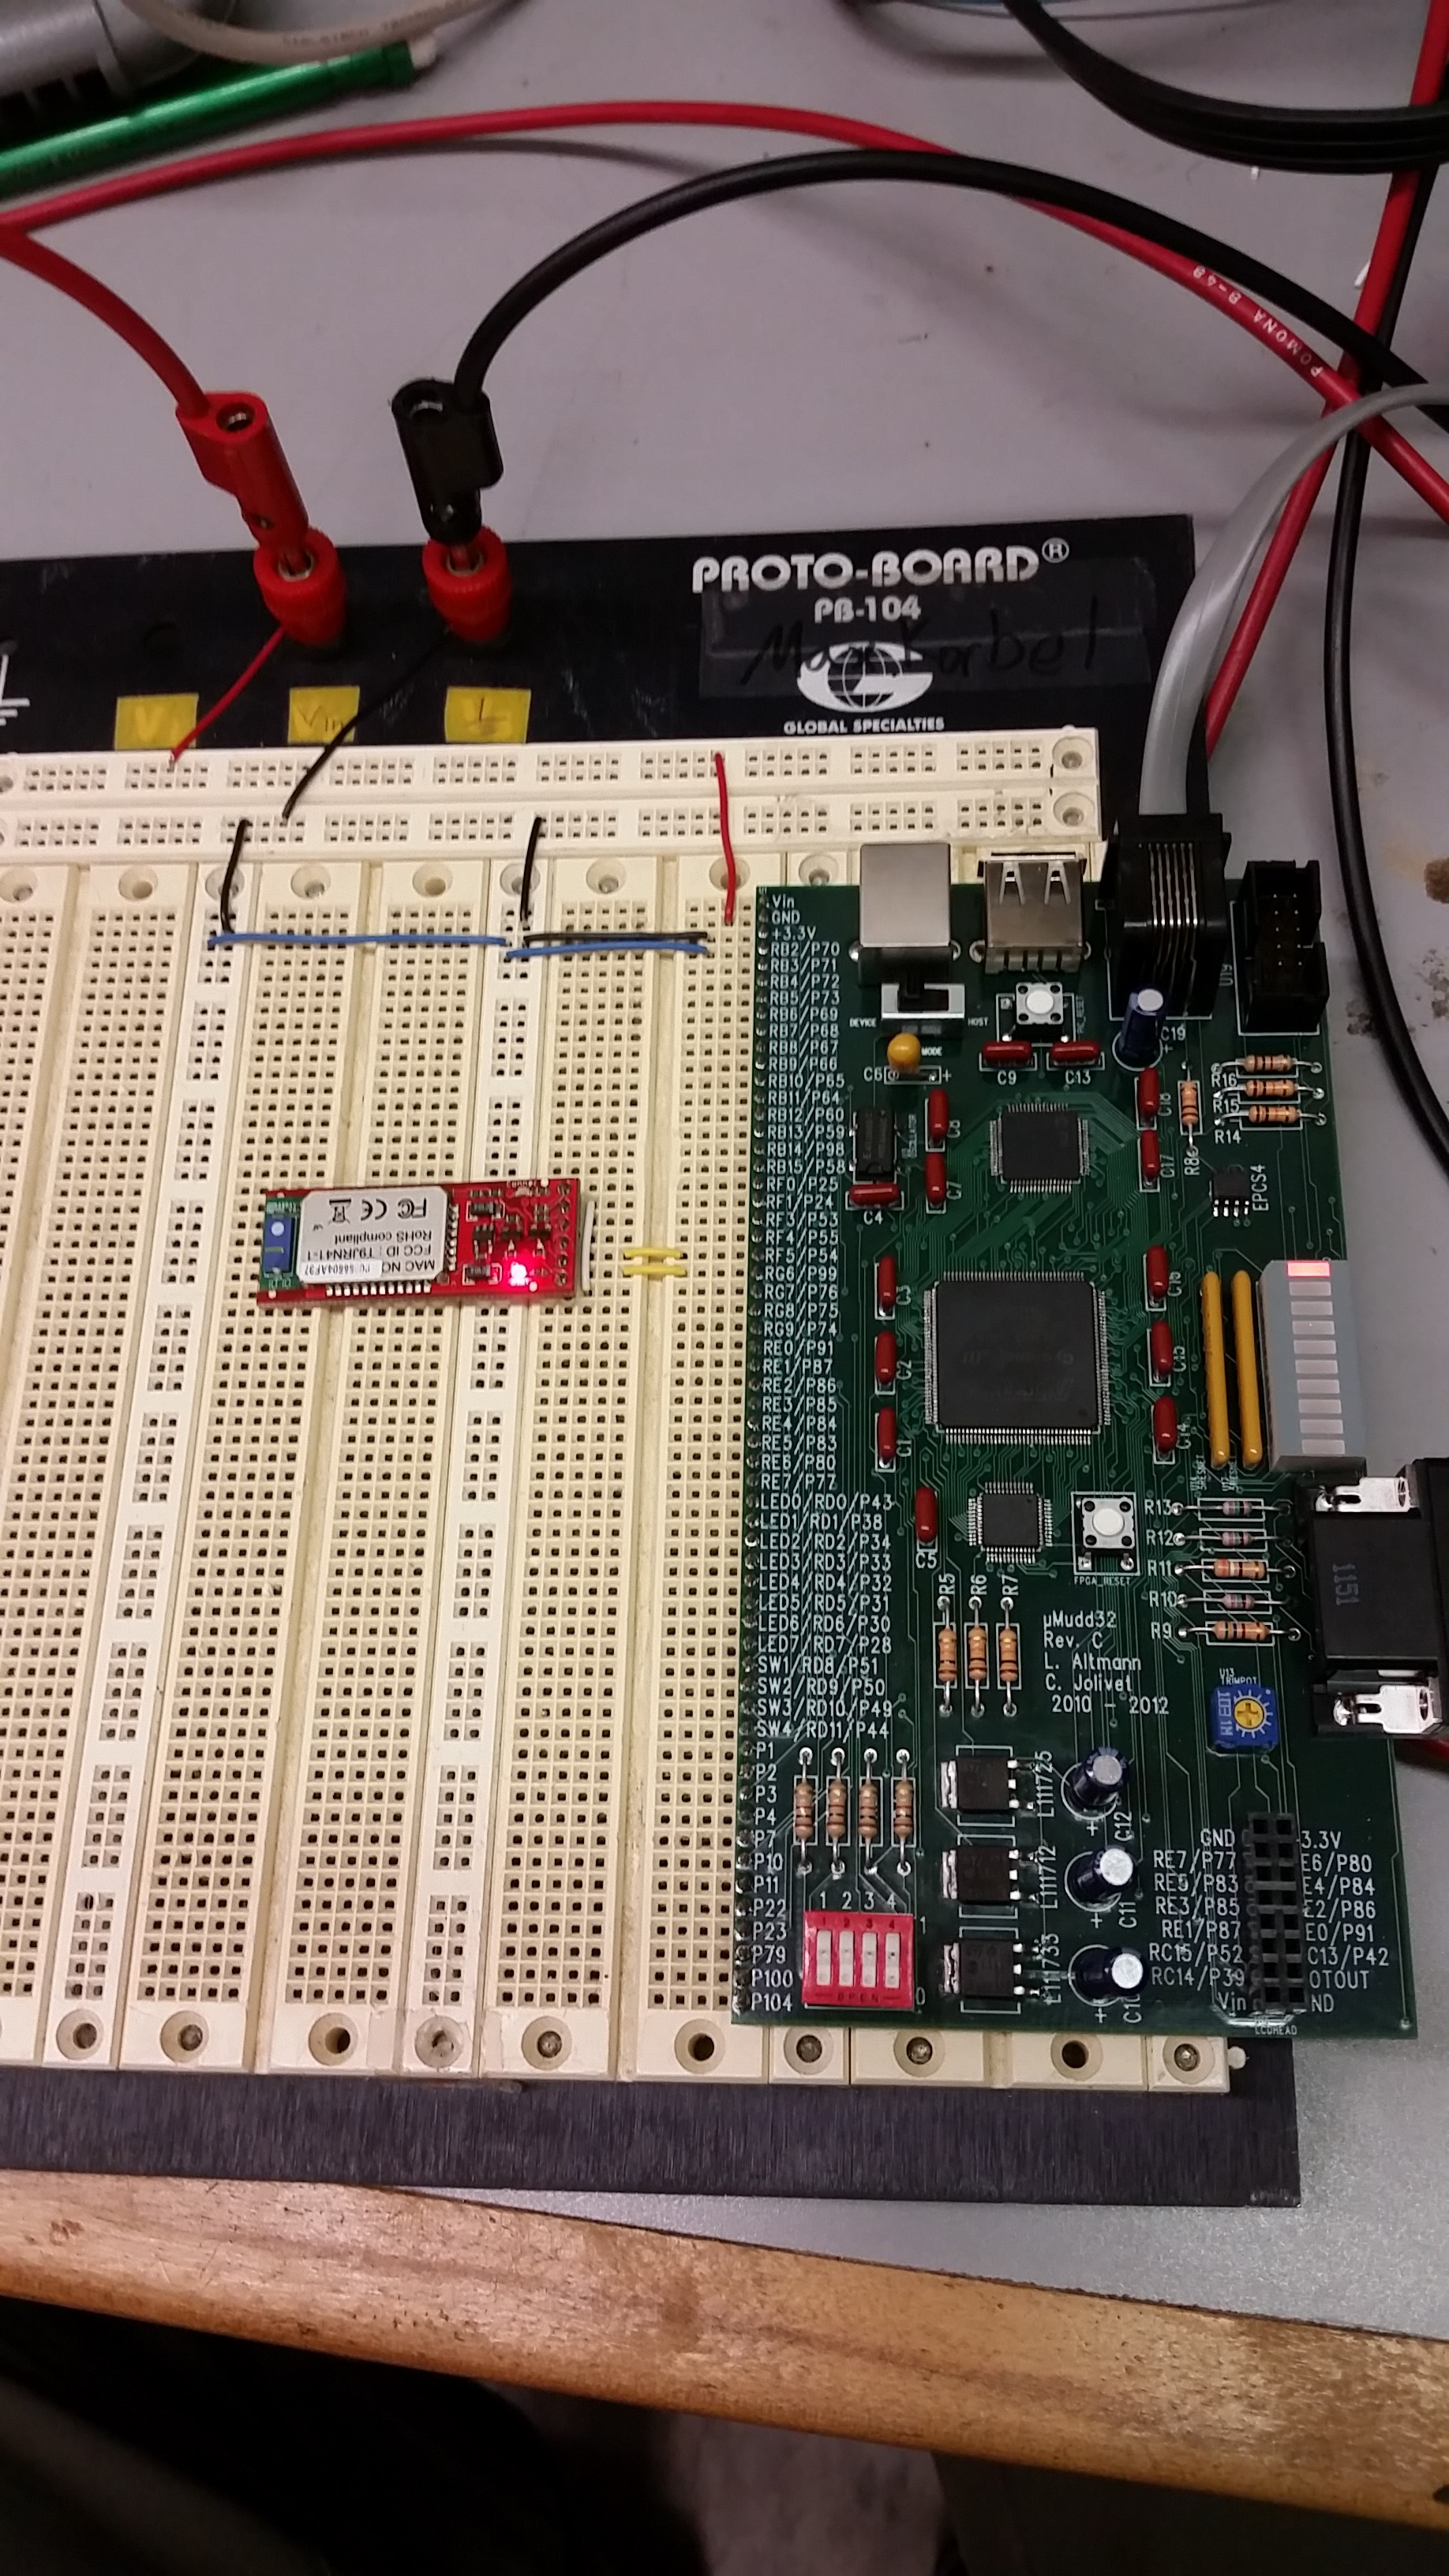
\includegraphics[scale=0.11]{board.jpg}
%\caption{The latest number entered on the keypad is displayed on the bottom display. The second latest number is displayed on the top.}
%\label{fig:board}
%\end{figure} 


\begin{document}



% ---------------------------------------
% Name section
% ---------------------------------------
\begin{flushleft}
Sherman Lam
\\E155
\\ \today
\end{flushleft}


% ---------------------------------------
% Title
% ---------------------------------------
\begin{center}
\begin{Large}
\textbf{Lab 4 Report: Microcontroller Sorting}
\end{Large}
\end{center}


% ---------------------------------------
% Start report
% ---------------------------------------


\section{Introduction}
\label{sec:intro}

In this lab, I implemented bubble sort in MIPS assembly. This was simulated in MPLAB-X and then tested on the PIC32 microcontroller located on the $\mu$Mudd32.



\section{Design and Testing Methodology}

\subsection{Sorting}

Instead of implementing a max finder for part c of the lab and then use selection sort for part d of the lab, I chose to implement bubble sort for part d. I then simply used the sorting algorithm to find the max for part c of the lab. While this is not the most efficient way (from a coding standpoint) to find the max of a list, it simplified the lab to use one main piece of source code. In addition, bubble sort is simpler to implement than selection sort. \\

Bubble sort is a very simple sorting algorithm. It is slow for sorting large lists but since we are sorting at most a list of 12 numbers, this algorithm is sufficient. In C, bubble sort is implemented as follows. \\

\begin{lstlisting}[numbers=left,basicstyle=\footnotesize]
bool flag;                              //1 = sorted, 0 = not sorted
int length = 12;                        //length of the list
while (flag != 1){                      //keep sorting if not sorted
    flag = 1;                           
    for (int i=0; i<length-1; i++){     
        n1 = array[i];                  //assume the list exists somewhere
        n2 = array[i+1];
        if (n1 > n2){
            pass;
        }
        else{                           //swap if they are out of order
            array[i] = n2;              
            array[i+1] = n1;
            flag = 0;                   //signal that list isn't sorted
        }
    }
}
\end{lstlisting}


\subsection{Using LEDs}

In order to control the LED with the PIC32, HIGH and LOW logic levels must be written to pins RD1 through RD7. These 8 pins are connected to the 8 lower LEDs on the $\mu$Mudd32. On the PIC32, pins RD1 through RD7 are part of a larger group of pins. Microchip gave this group of pins the designation "PORTD". In memory, the state of PORTD is simply stored as a 32-bit number. To change the outputs of any pin in PORTD, the PORTD bits in memory can be written to either 1 or 0. Notice though that while PORTD is stored as a 32-bit number, Figure \ref{fig:TRISD} shows that there are only 16 pins in PORTD and so only the bottom 16 bits of PORTD are used. \\

\begin{figure}[h!]
\centering
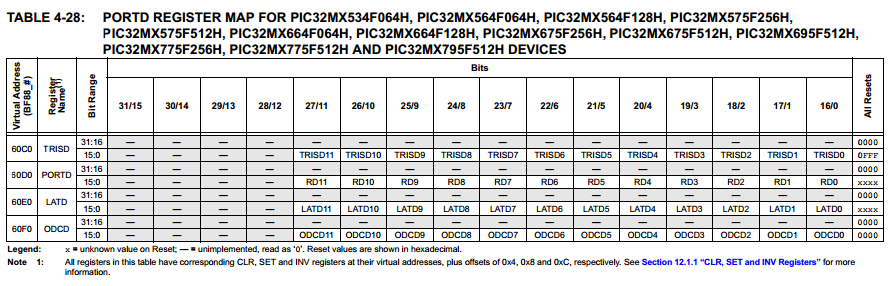
\includegraphics[scale=0.9,angle=90]{TRISD_and_PORTD.png}
\caption{Table from datasheet which shows which values of TRISD and PORTD are used. This also shows which pins PORTD is mapped to.}
\label{fig:TRISD}
\end{figure} 

However, to use these pins they must first be set to outputs or inputs. Those who have used an Arduino before will be familiar with this concept. On an Arduino, all pins must be set to inputs or outputs prior to use with the "pinmode" command. \\

PIC32 has a similar method of doing this. However, it operates at a lower level than Arduino. This is TRIS. Specifically, TRISD is used to control the mode of the pins in PORTD. TRISD is also a 32-bit number but only the bottom 16 bits are used (see Figure \ref{fig:TRISD} for the pin-to-bit mapping). When a bit in TRISD is 0, the corresponding pin is configured as an output, and vice versa (see PIC32 datasheet). 
 


\clearpage


\subsubsection{Simulation}

The following are some of the tests I ran to verify that the program was running correctly. On the left of each image is the list in the stack before it was sorted. The list on the right is the sorted list. Note that due to MPLAB and MPLAB-X's memory viewing system, larger addresses are towards the bottom. Since the stack grow from large to small addresses, the \enquote{top} of the stack is at the bottom of the image. So sorted lists will have the smallest number at the highest address / the bottom of the image / the top of the stack.

\begin{figure}[h!]
\centering
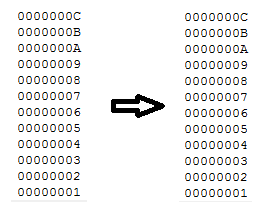
\includegraphics[scale=0.9]{sort1.png}
\caption{A sorted list should remain sorted.}
\label{fig:sort1}
\end{figure} 

\begin{figure}[h!]
\centering
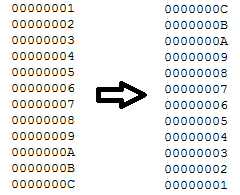
\includegraphics[scale=0.9]{sort2.png}
\caption{The sort works on a inverted list.}
\label{fig:sort2}
\end{figure} 

\begin{figure}[h!]
\centering
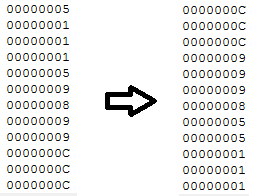
\includegraphics[scale=0.9]{sort3.png}
\caption{The sort works on a list of randomly selected numbers with repeats.}
\label{fig:sort3}
\end{figure} 

\begin{figure}[h!]
\centering
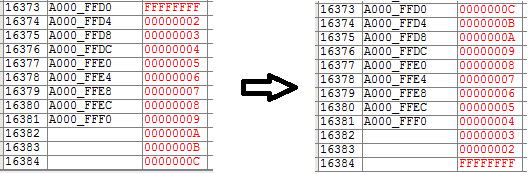
\includegraphics[scale=0.9]{sort4.png}
\caption{The sorts works on lists with negative numbers (in two's compliment).}
\label{fig:sort4}
\end{figure} 

\clearpage



\section{Technical Documentation}

\subsection{MIPS Code - Finding the Max}

\begin{lstlisting}[numbers=left,basicstyle=\footnotesize]
/*
This uses bubble sort to sort a list of 5, 32-bit numbers. It then
writes the largest number to the LEDs.

Author: Sherman Lam
Date: 10/5/14
Email: slam@g.hmc.edu
*/

#include <P32xxxx.h>    # header file that defines TRISD and PORTD

.global main            # start the main function

# Compiler instructions
.text           # store the code in the main program section of RAM
.set noreorder  # do not let the compiler reorganize your code

# define globals
#define LST1a   0x0
#define LST1b   0x1
#define LST2a   0x0
#define LST2b   0x2
#define LST3a   0x0
#define LST3b   0x3
#define LST4a   0x0
#define LST4b   0x4
#define LST5a   0x0000
#define LST5b   0x000F

#define PINMODE     0x0F00       # 1 = input, 0 = output


# Register use:
#   $t0 = counter (i)
#   $t1 = i*4
#   $t2 = slt results
#   $t3 = lower number (n1)
#   $t4 = upper number (n2)
#   $t5 = flag. 1 if list is sorted. 0 if not.
#   $t6 = 4
#   $t7 = stack pointer + i*4
#   $t8 = address of PORTD and TRISD
#   $s0 = 
#   $s1 = number to load / store to memory

.ent main

main:
    # load 5 numbers into the stack
    lui     s1, LST1a       # load first half of the number into reg
    ori     s1, LST1b       # load second half of the number into reg
    addi    sp, sp, -4      # add mem
    sw      s1, 0(sp)       # load number into ram
    lui     s1, LST2a       # load first half of the number into reg
    ori     s1, LST2b       # load second half of the number into reg
    addi    sp, sp, -4      # add mem
    sw      s1, 0(sp)       # load number into ram
    lui     s1, LST3a       # load first half of the number into reg
    ori     s1, LST3b       # load second half of the number into reg
    addi    sp, sp, -4      # add mem
    sw      s1, 0(sp)       # load number into ram
    lui     s1, LST4a       # load first half of the number into reg
    ori     s1, LST4b       # load second half of the number into reg
    addi    sp, sp, -4      # add mem
    sw      s1, 0(sp)       # load number into ram
    lui     s1, LST5a       # load first half of the number into reg
    ori     s1, LST5b       # load second half of the number into reg
    addi    sp, sp, -4      # add mem
    sw      s1, 0(sp)       # load number into ram

    # pin configuration
    la      t8, TRISD           # load the address of TRISD into t8
    addi    s1, zero, PINMODE   # load the pinmodes into s1
    sw      s1, 0(t8)           # set which pins are inputs or outputs.

    add     t5, zero, 0     # start a flag that indicates if the list is sorted.
    addi    t6, zero, 4     # load 4 into $t6
while:                      # start of while loop
    bne     t5, zero, done  # if $t5!=0, the list is sorted
    nop
    addi    t5, zero, 1     # set the flag to sorted
    add     t0, zero, zero  # init i at 0 
for:                        # start of for loop
    sltiu   t2, t0, 4       # make sure that the counter has not exceeded the length of the list
    beq     t2, zero, while # if the for loop is over, jump back to the while loop
    nop
    mul     t1, t0, t6      # calc i*4
    add     t7, sp, t1      # calc stack pointer + i*4
    lw      t3, 0(t7)       # load the number stored at the top of the stack (lowest addr) [n1]
    lw      t4, 4(t7)       # load the 2nd to last number [n2]
    add     t0, t0, 1       # increment the counter
    slt     t2, t3, t4      # check if n1 < n2 (out of order)
    beq     t2, zero, for   # pass if the numbers are in order ($t2=0)
    nop
    sw      t3, 4(t7)       # put n1 in n2's spot
    sw      t4, 0(t7)       # put n2 in n1's spot
    add     t5, zero, zero  # set the flag to 0 since the list is not sorted
    j       for
    nop
done:
    lw      s1, 0(sp)       # load the largest number in $s1
    la      t8, PORTD       # load the address of PORTD into $t8
    sw      s1, 0(t8)       # store the number in PORTD -> write to LEDs
    jr      ra              # return to function call
    nop

.end main

\end{lstlisting}


\subsection{MIPS Code - Sorting a List}

\begin{lstlisting}[numbers=left,basicstyle=\footnotesize]
/*
This uses bubble sort to sort a list of 12, 32-bit numbers

Author: Sherman Lam
Date: 10/5/14
Email: slam@g.hmc.edu
*/

.global main        # start the main function

# Compiler instructions
.text               # store the code in the main program section of RAM
.set noreorder      # do not let the compiler reorganize your code

# define globals
#define LST1a   0x0     # top 16 bits of the number
#define LST1b   0xC     # bottom 16 ibts of the number
#define LST2a   0x1     # top 16 bits of the number
#define LST2b   0xB     # bottom 16 ibts of the number
#define LST3a   0x0     # top 16 bits of the number
#define LST3b   0xA     # bottom 16 ibts of the number
#define LST4a   0x0     # top 16 bits of the number
#define LST4b   0x9     # bottom 16 ibts of the number
#define LST5a   0x0     # top 16 bits of the number
#define LST5b   0x8     # bottom 16 ibts of the number
#define LST6a   0x0     # top 16 bits of the number
#define LST6b   0x7     # bottom 16 ibts of the number
#define LST7a   0x0     # top 16 bits of the number
#define LST7b   0x6     # bottom 16 ibts of the number
#define LST8a   0x0     # top 16 bits of the number
#define LST8b   0x5     # bottom 16 ibts of the number
#define LST9a   0x0     # top 16 bits of the number
#define LST9b   0x4     # bottom 16 ibts of the number
#define LST10a  0x0     # top 16 bits of the number
#define LST10b  0x3     # bottom 16 ibts of the number
#define LST11a  0x0     # top 16 bits of the number
#define LST11b  0x2     # bottom 16 ibts of the number
#define LST12a  0xFFFF     # top 16 bits of the number
#define LST12b  0xFFFF     # bottom 16 ibts of the number

# Register use:
#   $t0 = counter (i)
#   $t1 = i*4
#   $t2 = slt results
#   $t3 = lower number (n1)
#   $t4 = upper number (n2)
#   $t5 = flag. 1 if list is sorted. 0 if not.
#   $t6 = 4
#   $t7 = ADDR + i*4
#   $t8 = 
#   $s0 = 
#   $s1 = number

.ent main

main:
    # load 12 numbers into the stack
    lui     $s1, LST1a      # load first half of the number into reg
    ori     $s1, LST1b      # load second half of the number into reg
    addi    $sp, $sp, -4    # add mem
    sw      $s1, 0($sp)     # load number into ram
    lui     $s1, LST2a      # load first half of the number into reg
    ori     $s1, LST2b      # load second half of the number into reg
    addi    $sp, $sp, -4    # add mem
    sw      $s1, 0($sp)     # load number into ram
    lui     $s1, LST3a      # load first half of the number into reg
    ori     $s1, LST3b      # load second half of the number into reg
    addi    $sp, $sp, -4    # add mem
    sw      $s1, 0($sp)     # load number into ram
    lui     $s1, LST4a      # load first half of the number into reg
    ori     $s1, LST4b      # load second half of the number into reg
    addi    $sp, $sp, -4    # add mem
    sw      $s1, 0($sp)     # load number into ram
    lui     $s1, LST5a      # load first half of the number into reg
    ori     $s1, LST5b      # load second half of the number into reg
    addi    $sp, $sp, -4    # add mem
    sw      $s1, 0($sp)     # load number into ram
    lui     $s1, LST6a      # load first half of the number into reg
    ori     $s1, LST6b      # load second half of the number into reg
    addi    $sp, $sp, -4    # add mem
    sw      $s1, 0($sp)     # load number into ram
    lui     $s1, LST7a      # load first half of the number into reg
    ori     $s1, LST7b      # load second half of the number into reg
    addi    $sp, $sp, -4    # add mem
    sw      $s1, 0($sp)     # load number into ram
    lui     $s1, LST8a      # load first half of the number into reg
    ori     $s1, LST8b      # load second half of the number into reg
    addi    $sp, $sp, -4    # add mem
    sw      $s1, 0($sp)     # load number into ram
    lui     $s1, LST9a      # load first half of the number into reg
    ori     $s1, LST9b      # load second half of the number into reg
    addi    $sp, $sp, -4    # add mem
    sw      $s1, 0($sp)     # load number into ram
    lui     $s1, LST10a     # load first half of the number into reg
    ori     $s1, LST10b     # load second half of the number into reg
    addi    $sp, $sp, -4    # add mem
    sw      $s1, 0($sp)     # load number into ram
    lui     $s1, LST11a     # load first half of the number into reg
    ori     $s1, LST11b     # load second half of the number into reg
    addi    $sp, $sp, -4    # add mem
    sw      $s1, 0($sp)     # load number into ram
    lui     $s1, LST12a     # load first half of the number into reg
    ori     $s1, LST12b     # load second half of the number into reg
    addi    $sp, $sp, -4    # add mem
    sw      $s1, 0($sp)     # load number into ram
    
    add     $t5, $0, $0     # start a flag that indicates if the list is sorted.
    addi    $t6, $0, 4      # load 4 into $t6
while:                      # start of while loop
    bne     $t5, $0, done   # if $t5!=0, the list is sorted
    nop
    addi    $t5, $0, 1      # set the flag to sorted
    add     $t0, $0, $0     # init i at 0 
for:                        # start of for loop
    sltiu   $t2, $t0, 11    # make sure that the counter has not exceeded the length of the list
    beq     $t2, $0, while  # if the for loop is over, jump back to the while loop
    nop
    mul     $t1, $t0, $t6   # calc i*4
    add     $t7, $sp, $t1   # calc stack pointer + i*4
    lw      $t3, 0($t7)     # load the number stored at the top of the stack (lowest addr) [n1]
    lw      $t4, 4($t7)     # load the 2nd to last number [n2]
    add     $t0, $t0, 1     # increment the counter
    slt     $t2, $t3, $t4   # check if n1 < n2 (out of order)
    beq     $t2, $0, for    # pass if the numbers are in order ($t2=0)
    nop
    sw      $t3, 4($t7)     # put n1 in n2's spot
    sw      $t4, 0($t7)     # put n2 in n1's spot
    add     $t5, $0, $0     # set the flag to 0 since the list is not sorted
    j       for
    nop
done:
    
    jr      $ra             # return to function call
    nop

.end main
\end{lstlisting}


\section{Results and Discussion}

The sorting works! For part c of the lab, the max number is successfully displayed on the LEDs. For part d of the lab, the sorted list can be monitored through MPLAB-X's memory viewer.


\section{Conclusion}

\subsection{Time Spent}

\begin{description}
	\item[Programming, Simulating] 5hrs
	\item[Writing Report] 2.5hrs
	\item[Total Time Spent] 7.5hrs
\end{description}

\subsection{Suggestions for lab}

Use MPLAB-X instead of MPLAB. The interface is easier to use, cleaner, and not as buggy. Writing a lab to use MPLAB-X would be helpful.

\end{document}

